Kiến trúc vi dịch vụ có nhiều ưu điểm, đặc biệt với các dự án có quy mô lớn và phức tạp.

\begin{itemize}

    \item Kiến trúc vi dịch vụ phân chia dự án thành các dịch vụ nhỏ.

          \begin{itemize}

              \item Giúp việc phát triển và quản lý dễ dàng hơn.

              \item Tận dụng sử dụng tài nguyên theo nhu cầu cho từng dịch vụ riêng.


          \end{itemize}

    \item Các dịch vụ trong kiến trúc vi dịch vụ  độc lập về nghiệp vụ kinh doanh, ngôn ngữ lập trình, CSDL, triển khai hệ thống,...

\end{itemize}
% Bối cảnh giới hạn : Kiến trúc phải được thiết kế để phù hợp với ranh giới của khả năng kinh doanh, sao cho mỗi dịch vụ chịu trách nhiệm về một tập hợp chức năng cụ thể, gắn kết.
Các nhóm  không cần phải đi sâu vào mọi khả năng kinh doanh từ đó dẫn đến tốc độ định giá doanh nghiệp nhanh hơn.
Các nhóm phát triển riêng dẫn tới tốc độ phát triển thay đổi nhanh.
% Tự chủ : Các dịch vụ phải có khả năng hoạt động tự chủ, ít phụ thuộc vào các dịch vụ khác.






% Khả năng mở rộng  hệ thống   dễ dàng.



% Triển khai độc lập : Mỗi dịch vụ phải có khả năng triển khai độc lập để có thể thực hiện các thay đổi đối với một dịch vụ mà không ảnh hưởng đến các dịch vụ khác.




Giảm thiểu ràng buộc và tăng tính linh hoạt của hệ thống.

Giảm chi phí và thời gian kiểm thử do ít ràng buộc.

Hệ thống có khả năng chịu lỗi cao tăng độ tin cậy.
% Khả năng phục hồi : Kiến trúc phải được thiết kế để chịu đựng lỗi và các dịch vụ phải có khả năng xử lý lỗi một cách duyên dáng.

%%%%%%%%%%%%%%%%%%%%%%%%%%%%%%%%%%%%%
Tính linh hoạt : Kiến trúc phải cho phép phát triển và triển khai nhanh chóng các dịch vụ mới cũng như khả năng thay đổi các dịch vụ hiện có một cách nhanh chóng và dễ dàng.



 

Kiến trúc vi dịch vụ sử dụng đa ngôn ngữ và công nghệ khác nhau.

Tận dụng hiệu quả thế mạnh của từng ngôn ngữ, công nghệ phù hợp nhất cho yêu cầu nghiệp vụ cụ thể.

% Ví dụ: Mỗi dịch vụ sử dụng ngôn ngữ lập trình nhau khác như: NodeJS, Go, Python, Java, CSharp,...

% \begin{figure}[h]
    
    % \centering
    
    % 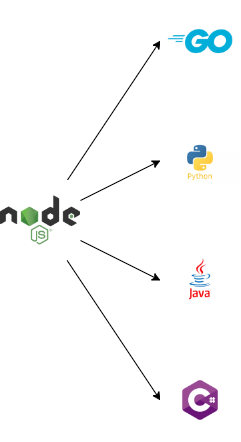
\includegraphics[height = 3cm]{pictures/DaNgonNgu/_DaNgonNgu.png}
    
    % % \caption{ViDuHinhAnhTheoChieuDoc}
    
    % Thêm vào hình SQL riêng
    
    % \end{figure}
    
    
    % Các dịch vụ tương tác với nhau qua hạ tầng mạng.
    % Các dịch vụ tương tác với nhau qua hạ tầng mạng.
    % Các dịch vụ tương tác với nhau qua hạ tầng mạng.
    % Các dịch vụ tương tác với nhau qua hạ tầng mạng.
    % Các dịch vụ tương tác với nhau qua hạ tầng mạng.
    % Các dịch vụ tương tác với nhau qua hạ tầng mạng.
    % Các dịch vụ tương tác với nhau qua hạ tầng mạng.
    % Các dịch vụ tương tác với nhau qua hạ tầng mạng.
    % Các dịch vụ tương tác với nhau qua hạ tầng mạng.